%----------------------------------------------------------------------------------------
%	SECTION 1.1
%----------------------------------------------------------------------------------------

\section{Compact Spaces.}

\begin{definition}
    A collection $\Ac=\{A_{\alpha}\}$ of subsets of a topological space $X$ is said to be a  \textbf{cover}, or a
    \textbf{covering} of $X$ if  $X \subseteq \bigcup{A_\alpha}$. We call
    $\{A_\alpha\}$ an \textbf{open cover} if each $A_\alpha$
    is open in  $X$. If  $\{A'_\alpha\}$ is a subcollection of $\Ac$ that also covers $X$, we call
    $\{A'_\alpha\}$ a \textbf{subcover} of $X$.
\end{definition}

\begin{definition}
    We call a topological space $X$ \textbf{compact} if for every open cover of $X$, there is a
    finite subcover of $X$.
\end{definition}

\begin{example}
    \begin{enumerate}
        \item[(1)] $\R$ is not compact. Consider the following cover of  $\R$:
            \begin{equation*}
                \Ac=\{(n,n+2):n \in \Z\}
            \end{equation*}
            however, there is no finite subcollection of $\Ac$ that is a subcover of  $\R$.

        \item[(2)] The subspace $X=\{0\} \cup \{\frac{1}{n}: n \in \Z\}$ of $\R$ is compact. Let  $\Ac$
            be a cover of  $X$. There is a  $U \in \Ac$ with  $0 \in U$ and $U$ contains all but
            finitely many of the points  $ \frac{1}{n}$. Now choose for each $\frac{1}{n} \in
            \com{X}{U}$ an element of $\Ac$ $A_{n}$ containing it. Then for all $n$,  $\{A_n\}$ is
            finite and covers $X$.

        \item[(3)] If  $X$ is a finite topological space, then it is compact, since every open cover of
            $X$ is finite.

        \item[(4)] The interval  $(0,1]$ is not compact. The open cover $\Ac=\{(\frac{1}{n}, 1]: n \in
            \Z^+\}$ contains no finite subcollection of $\Ac$ that covers  $(0,1]$. Likewise,
            $(0,1)$ is not compact by the same argument. However, $[0,1]$ is compact.
    \end{enumerate}
\end{example}

\begin{lemma}\label{3.4.1}
    Let $Y$ be a subspace of a topological space  $X$.  $Y$ is compact if and only if every open
    cover of  $Y$, by open sets of  $X$ has a finite subcover of $Y$.
\end{lemma}
\begin{proof}
    Suppose $Y$ is compact and let  $\{A_\alpha\}$ be a cover of $Y$ with  $A_\alpha$ open in  $X$
    for all  $\alpha$. Since  $\{A_\alpha\}$ covers $Y$, so does the collection  $\{A_\alpha \cap
    Y\}$, where $A_\alpha \cap Y$ is open in  $Y$ for all  $\alpha$. Since  $Y$ is compact, choose
    the finite subcollection  $\{A_i \cap Y\}_{i=1}^{n}$ to be a finite subcover of $Y$; i.e.
    $\{A_i \cap Y\}_{i=1}^{n} \subseteq \{A_\alpha\}$.

    Conversely, suppose that for every cover $\{A_\alpha\}$, open in  $X$, of  $Y$ that
    $\{A_\alpha\}$ contains a finite subcover of $Y$. Choose  $A_\alpha'=A_\alpha \cap Y$ for all
    $\alpha$; then $\{A_\alpha'\}$ is an open cover of $Y$.
    By hypothesis, there is a finite subcover $\{A_i\}_{i=1}^n$, and by our assignment, we
    get that $\{A_i'\}_{i=1}^n \subseteq \{A_\alpha'\}$ is also a finite subcover of $Y$. Therefore
     $Y$ is compact as a subspace of  $X$.
\end{proof}

\begin{theorem}\label{3.4.2}
    Every closed subspace of a compact space is compact.
\end{theorem}
\begin{proof}
    Let $Y$ be a closed subspace of a compact space $X$. Let $\{A_\alpha\}$ be an open cover of $Y$
    with  $A_\alpha$ open in  $X$ for all  $\alpha$. Consider  $\{B_\alpha\}=\{A_\alpha\} \cup
    \com{X}{Y}$. Since $\{A_\alpha\}$ covers $Y$,  $\{B_\alpha\}$ covers $X$. Now take some finite
    subcollection  $\{B_i\}_{i=1}^n$. If it contains $\com{X}{Y}$, then just consider
    $\com{\{B_i\}}{(\com{X}{Y})}$. Then this collection is a finite subcover of $Y$.
\end{proof}

\begin{theorem}\label{3.4.3}
    Every compact subspace of a Hausdorff space is closed.
\end{theorem}
\begin{proof}
    Let $Y$ be a compact subsapce of a Hausdorff space  $X$. Choose  $x_0 \in \com{X}{Y}$ and for
    each $y \in Y$ choose disjoint neighborhoods  $U_y$ and  $V_y$ of  $ x_0$ and $y$ respectively.
    The collection  $\{V_y\}$ covers $Y$ by open sets in  $X$, hence there is a finite subcover, by
    theorem \ref {3.4.2}, $\{V_{y_n}\}$ of $Y$. Take  $V=\bigcup_{i=1}^n{V_{y_i}}$ to be open in
$X$, and take  $U=\bigcap_{i=1}^n{U_{y_i}}$ also open in $X$. Then  $Y \subseteq V$ and  $V \cap
U=\emptyset$; for take $z \in V$,  $z \in V_{y_i}$ for some $1 \leq i \leq n$. Hence  $z \notin
U_{y_i}$, so $z \notin U$. Then  $U$ is a neighborhood of  $X$, disjoint from  $Y$, making
$\com{X}{Y}$ open in $X$. Therefore  $Y$ is closed in  $X$.
\end{proof}

\begin{figure}[h]
    \centering
    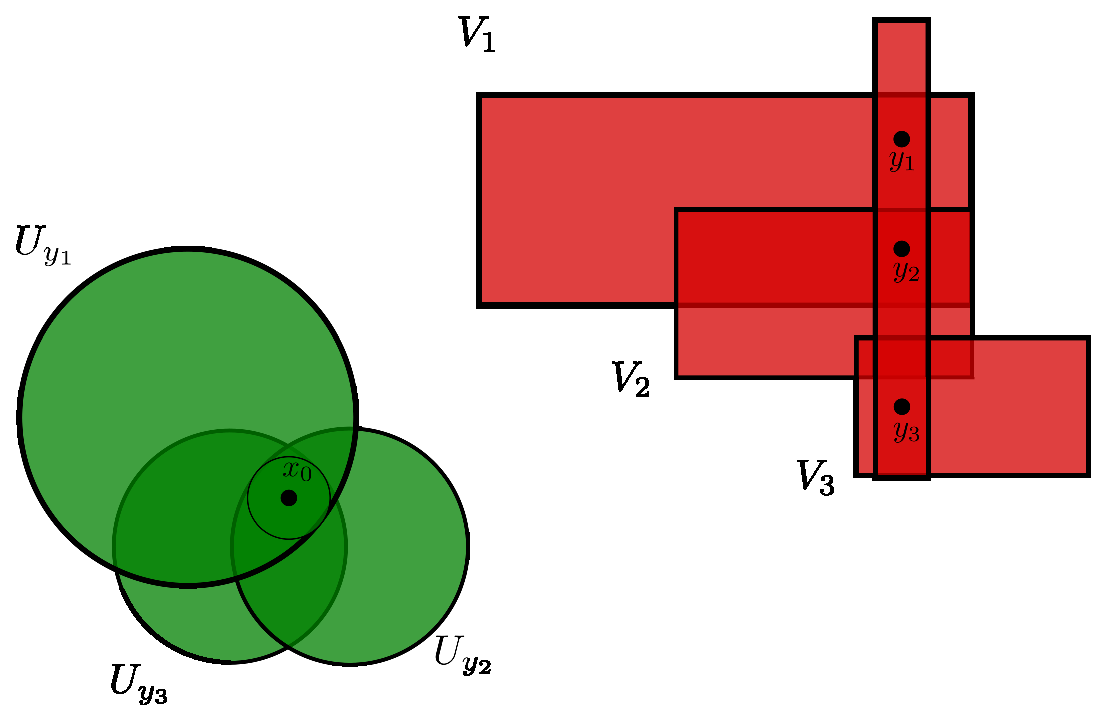
\includegraphics[scale=0.5]{Figures/chapter3/compact_hausdorf_space.eps}
    \caption{Closed sets of a compact Hausdorff space (See theorem \ref{3.4.3}).}
    \label{fig_3.1}
\end{figure}

\begin{corollary}
    If $Y$ is a compact subspace of a Hausdorff space $X$, and  $ x_0 \in \com{X}{Y}$, then there
    exists opensets $U$ and  $V$ in  $X$ with  $ x_0 \in U$ and $Y \subseteq V$, respectively.
\end{corollary}

\begin{example}
    \begin{enumerate}
        \item[(1)] Since $[a,b]$ is compact in $\R$, so is any closed subspace of  $[a,b]$. The
            subspaces $(a,b]$, $[a,b)$, and $(a,b)$, however, are not compact; as they are not
            closed in $\R$ as a Hausdorff space.

        \item [(2)] Consider the finite complement topology on $\R$. Every proper finite subset of
            $\R$ is closed under finite complements, however every subset of  $\R$ is compact in the
            finite complement topology.
    \end{enumerate}
\end{example}

\begin{theorem}\label{3.4.4}
    If $X$ is a compact space, and  $Y$ is a topological space, and  $f:X \rightarrow Y$ is a
    continuous map, then $f(X)$ is compact.
\end{theorem}
\begin{proof}
    Let $f:X \rightarrow Y$ be continuous, and let $X$ be compact. Let  $\Cc$ be a cover of  $f(X)$
    by sets ib $Y$, and consider the collection  $\{f^{-1}(C)\}_{C \in \Cc}$. We have that
    $f^{-1}(C)$ is open in $X$ by continuity, hence there is a finite subcollection
    $\{f(C_i)\}_{i=1}^n$ covering $X$  (by compactness) That is $X \subseteq
    \bigcup_{i=1}^n{f(C_i)}$, hence $f(X) \subseteq \bigcup{C_i}$, which makes $\{C_i\}_{i=1}^n$ a
    finite subcover of $f(X)$.
\end{proof}

\begin{theorem}\label{3.4.5}
    Let $X$ be compact, and  $Y$ be Hausdorff, and let  $f:X \rightarrow Y$ be a $1-1$ continuous
    map of  $X$ onto  $Y$. Then  $f$ is a homomorphism.
\end{theorem}
\begin{proof}
    If $A \subseteq X$ is closed, then  $A$ is compact by theorem \ref {3.4.2}, making $f(X)$
    compact in $Y$. Since  $Y$ is Hausdorff,  $f(A)$ closed is in $Y$. This makes $f^{-1}$
    continuous.
\end{proof}

\begin{definition}
    Let $X$ be a topological space and let  $Y$ be compact. Let  $x_0 \in X$ and $N \subseteq X
    \times Y$. If  $W$ is a neighbourhood of  $x_0 \times Y$ such that $W \times Y \subseteq N$,
    then we call  $W \times Y$ a  \textbf{tube} about $x_0 \times Y$.
\end{definition}

The following theorem lemma states the existence of such tubes, and helps establish the next theorem

\begin{lemma}[The Tube Lemma]\label{3.4.6}
    Let $X$ be a topological space, and let  $Y$ be compact. Choose  $x_0 \in X$ and $N \subseteq X
    \times Y$ open. Then there exists a tube  $W \times Y$ about  $x_0 \times Y$, for some
    nieghbourhood $W$ of  $x_0$.
\end{lemma}
\begin{proof}
    Take $x_0 \in X$ and let $N \subseteqX \times Y$ be open. We show there
    exists a tube about $x_0 \times Y$. Cover $x_0 \times Y$ by basis elements
    $U \times V \subseteq N$. We have  $x_0 \times Y$ is compact since
    $x_0 \times Y$ is homeomorphic to $Y$; hence there is a finite subcollection
    $\{U_i \times V_i\}_{i=1}^n$ of the $U \times V \subseteq N$ covering  $x_0
    \times Y$, supposing that $U_i \times V_i$ intersects  $x_0 \times Y$ for
    all $i$. Now define $W=\bigcap_{i=1}^n{U_i}$. $W$ is open in  $X$, and
    contains  $x_0$.

    Now let x \times y \in $W \times Y$ and  $x_0 \times y \in x_0 \times Y$.
    We have that $x_0 \times y \in U_i \times v_i$, hence $y \in V_i$ for
    $1 \leq i \leq n$. We also get that  $x \in U_j$ for all  $1 \leq j \leq n$,
    since  $x \in W$ by definition. Hence  $x \times y \in U_i \times V_i$.
    Since  $W \subseteq U_i \times V_i \subseteq N$, for all  $1 \leq i \leq n$,
    we get the required result.
\end{proof}

\begin{theorem}\label{3.4.7}
    Finite products of compact spaces are compact.
\end{theorem}
\begin{proof}
    Let $\Cc$ be an open cover of  $X \times Y$, with  $X$ and  $Y$ compact. Take  $x_0 \in X$ and
    consider $x_0 \times Y$ compact in $X \times Y$. Then  $x_0 \times Y$ can be covered by a finite
    subcollection $\{C_i\}_{i=1}^n \subseteq \Cc$. Take $N=\bigcup_{i=1}^n{C_i}$. Then $x_0 \times Y
    \subseteq N$. By the tube lemma, there is a tube $W \times Y$ about  $x_0 \times Y$ with $W$ a
    neighbourhood of  $x_0$, so $W \times Y \subseteq N$.

    Now for each $x \in X$, choose  $W_x$ such that  $W_x \times Y$ can be covered by a finite
    subcollection of  $\Cc$. $\{W_x\}$ forms an open cover of $X$, hence by compactness there is a
    finite subcover of  $X$  $\{W_i\}_{i=1}^n \suseteq \{W_x\}$. Take $\{W_i \times Y\}_{i=1}^n$ and
    their union contains $X \times Y$.
\end{proof}

\begin{example}
    Let $Y=0 \times \R$ and let  $N=\{x \times y: |x|<\frac{1}{y^2+1}\}$. $N$ is open in  $\R^2$ and
     $Y \subseteq N$; however there is no tube about  $Y$, so the tube lemma fails when  $Y$ is not
     compact.
\end{example}

\begin{definition}
    A collection $\Cc$ of subsets of a set  $X$ is said to satisfy the  \textbf{finite intersection
    property} (or \textbf{FIP}) if every for finite subcollection $\{C_i\}_{i=1}^n$ of $\Cc$,
    $\bigcap_{i=1}^n{C_i} \neq \emptyset$.
\end{definition}

\begin{theorem}\label{3.4.8}
    Let $X$ be a topological space.  $X$ is compact if and only if for every collection  $\Cc$ of
    closed sets satisfying the FIP, the intersection $\bigcap_{C \in \Cc}{C} \neq \emptyset$.
\end{theorem}
\begin{proof}
    Let $\Ac$ be a collection of subsets of  $X$, and define  $\Cc=\{\com{X}{A}:A \in \Ac\}$. The
    following hold:
    \begin{enumerate}
        \item[(1)] $\Ac$ is a collection of open sets if and only if $\Cc$ is a collection of closed
            sets.

        \item [(2)] $\Ac$ covers  $X$ if and only if  $\bigcap_{C \in \Cc}{C}=\emptyset$.

        \item[(3)] A finite subcollection $\{A_i\}_{i=1}^n$ of $\Ac$ covers  $X$ if and only if
            $\bigcap{\com{X}{A_i}}=\emptyset$.
    \end{enumerate}
    Take the contrapositive and then the complements of the sets.
\end{proof}
